%=========================================================================
% (c) 2014, 2015 Josef Lusticky

\section{Spirent configuration}
Custom iMix, named AMS-IX, was configured acording to the AMS-IX statistics described in section~\ref{sec:analysis-metodology}.
Figure~\ref{fig:setup-amsix-imix} shows the configuration window for custom iMix definiton
from the Spirent TestCenter Application.
One device was configured on each interface and it was assigned IPv4 and IPv6 adddress, as described in section~\ref{sec:setup-hardware}.
The {\it{Respond to ping}} option was enabled to test the connection.
Two traffic patterns were configured - one for IPv4 traffic and the other for IPv6 traffic. %TODO - patterns
\begin{figure}
	\centering
	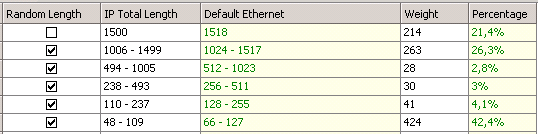
\includegraphics[width=14.5cm,keepaspectratio]{fig/amsix-imix.png}
	\caption{AMS-IX iMix}
	\label{fig:setup-amsix-imix}
\end{figure}

To test the routing performance of the Linux kernel with full BGP table, 
another scenario was configured.
%TODO - scenario, dopsat vetu, pridat konfiguraci
